\documentclass[12pt]{book}

%These tell TeX which packages to use.
\usepackage{array,epsfig}
\usepackage{amsmath}
\usepackage{amsfonts}
\usepackage{amssymb}
\usepackage{amsxtra}
\usepackage{amsthm}
\usepackage{mathrsfs}
\usepackage{color}
\usepackage{eurosym}
\usepackage{times}
%Here I define some theorem styles and shortcut commands for symbols I use often
\theoremstyle{definition}
\newtheorem{defn}{Definition}
\newtheorem{thm}{Theorem}
\newtheorem{cor}{Corollary}
\newtheorem*{rmk}{Remark}
\newtheorem{lem}{Lemma}
\newtheorem*{joke}{Joke}
\newtheorem{ex}{Example}
\newtheorem*{soln}{Solution}
\newtheorem{prop}{Proposition}

\newcommand{\lra}{\longrightarrow}
\newcommand{\ra}{\rightarrow}
\newcommand{\surj}{\twoheadrightarrow}
\newcommand{\graph}{\mathrm{graph}}
\newcommand{\bb}[1]{\mathbb{#1}}
\newcommand{\Z}{\bb{Z}}
\newcommand{\Q}{\bb{Q}}
\newcommand{\R}{\bb{R}}
\newcommand{\C}{\bb{C}}
\newcommand{\N}{\bb{N}}
\newcommand{\M}{\mathbf{M}}
\newcommand{\m}{\mathbf{m}}
\newcommand{\MM}{\mathscr{M}}
\newcommand{\HH}{\mathscr{H}}
\newcommand{\Om}{\Omega}
\newcommand{\Ho}{\in\HH(\Om)}
\newcommand{\bd}{\partial}
\newcommand{\del}{\partial}
\newcommand{\bardel}{\overline\partial}
\newcommand{\textdf}[1]{\textbf{\textsf{#1}}\index{#1}}
\newcommand{\img}{\mathrm{omega}}
\newcommand{\ip}[2]{\left\langle{#1},{#2}\right\rangle}
\newcommand{\inter}[1]{\mathrm{int}{#1}}
\newcommand{\exter}[1]{\mathrm{ext}{#1}}
\newcommand{\cl}[1]{\mathrm{cl}{#1}}
\newcommand{\ds}{\displaystyle}
\newcommand{\vol}{\mathrm{vol}}
\newcommand{\cnt}{\mathrm{ct}}
\newcommand{\osc}{\mathrm{osc}}
\newcommand{\LL}{\mathbf{L}}
\newcommand{\UU}{\mathbf{U}}
\newcommand{\support}{\mathrm{support}}
\newcommand{\AND}{\;\wedge\;}
\newcommand{\OR}{\;\vee\;}
\newcommand{\Oset}{\varnothing}
\newcommand{\st}{\ni}
\newcommand{\wh}{\widehat}

%Pagination stuff.
\setlength{\topmargin}{-.3 in}
\setlength{\oddsidemargin}{0in}
\setlength{\evensidemargin}{0in}
\setlength{\textheight}{9.in}
\setlength{\textwidth}{6.5in}
\pagestyle{empty}

\begin{document}

\begin{center}
{\Large DATA 221 \\  Homework 3  (rev 1)}\\
\textbf{Trimble/Nussbaum}\\ %You should put your name here
Due: Friday 2023-01-26 11:59pm
\end{center}

\vspace{0.2 cm}

This question asks to you produce a graph like of overfitting given in Hastie Elements of Statistical Learning Figure 2.4.  The underlying source of the points in the graph was a lumpy mixture of normal distributions.  We will have to generate random parameters for this distribution, generate samples from the distribution for training, and generate another (large) set of samples for testing.  The random dataset you generate should look like a shotgun target.

To start, you need to make a distribution of 100 orange and 100 blue points.  Start by generating  10 means for class 1 (orange) and 10 means for class 2 (blue) from a normal distribution with variance (1, 1) and centered at ($x_1$ ,$x_2$) = (0,1) for blue and (1,0) for orange and no correlation between $x_1$ and $x_2$.   
For the trainign data, generate 10 data points from a 2d normal with standard deviation 1/3 for each (of the 20) clusters.  This is now a lumpy distribution in two dimensions with 10 clusters for class 1 and 10 clusters for class 2.

% Be ready to generate more 10,000 samples form these distributions; keep track of the cluster means since you will need them later.

\begin{enumerate}
\item 
Generate 200 points from the lumpy-Gaussian-mixture dataset as described above.  Plot a scatterplot.

\item
Visualize the Bayes decision boundary between the two classes, the surfaces where the (true) density in class 1 equals the density in class 2.  You can use contour maps to approximate the boundary or you can solve for the boundaries numerically.

\item
Generate a large "testing" sample of 10,000 points from this lumpy distribution.
Estimate the accuracy of the Bayes classifier trained on the 200-point training set by counting how many of the testing set are classified correctly.  This number depends on your random values; some instances have larger and smaller amounts of irreducible error.

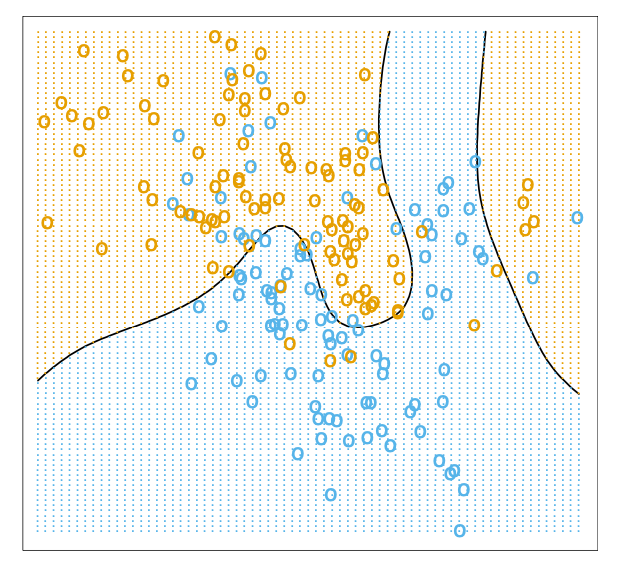
\includegraphics[width=3in]{src/hastie-bayesian.png}

%\item
%Perform K-nearest-neighbor classification for at least six values of $k$ ranging from 1 to 100; use the neighbors of each point to predict the class identity.  Evaluate accuracy as a function of $k$ for the training set (with 200 points).

%\item
%Generate a large "testing" sample of 10,000 points from each class.
%Evaluate the accuracy of KNN classification (trained on the 200-point training set)  as a function of $k$ for the 20,000 points in the test set and plot the accuracy vs. $k$ for the training and the testing data on the same graph.   

%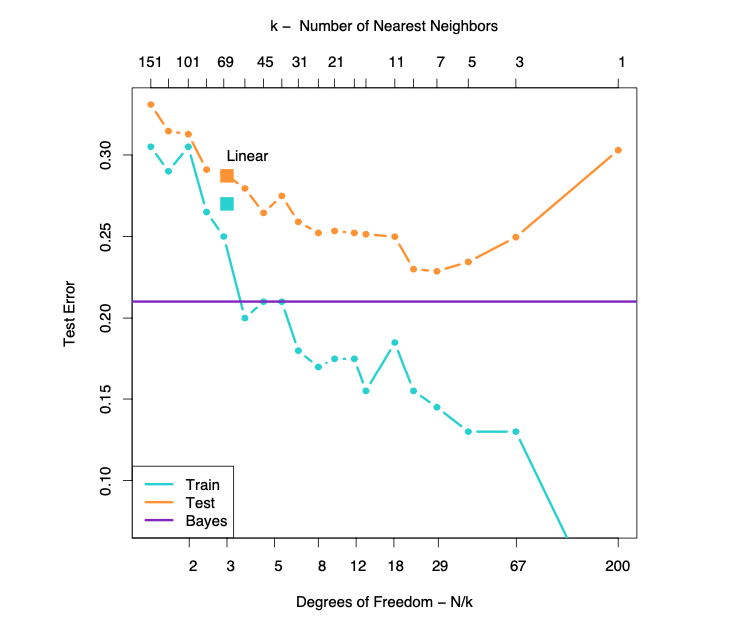
\includegraphics[width=4in]{hastie-generalization.png}

The UCI "default of credit card clients Data Set" contains various fields describing 30,000 credit card customers in Taiwan in 2005. (Yeh \& Lien,  doi://10.1016/j.eswa.2007.12.020)   

\item
Split the dataset 50/50 into training and test, and try several logistic regression models to predict the \texttt{default.payment.next.month} field.  


\item
Present a summary of a handful of the models that gave the best accuracy on the test set.  Which variables did you include, and which ones mattered the most?

%\item 
%Try to predict the \texttt{default.payment.next.month} using KNN classifiers for four different values of $k$.

%You have to choose how to measure distance in a vector space that includes indicator variables and payment amounts (\$NT 100k).  

%Report accuracy on the testing and training datasets.

\texttt{https://archive.ics.uci.edu/ml/datasets/default+of+credit+card+clients}

\end{enumerate}
\end{document}


